\documentclass{ctexart}
\usepackage[hmargin=1.1in,vmargin=1in]{geometry}
\usepackage{amsmath}
\usepackage{graphicx}
\usepackage[defaultmono]{droidsansmono}

\title{《信号处理导论》课程报告六}
\input{personal_info/info.tex}

\begin{document}
    \maketitle

    \section{我学到了哪个知识点?}

    系统的描述。系统可以使用框图和数学模型来描述。其中连续系统的数学模型是微分方程,离散系统的数学模型是差分方程。
    而一个即时系统可以直接使用一个代数方程来描述。框图中系统的各个部件可以用一些符号来表示,通常我们不关系这些部件
    的内部结构(绘制框图时我们不会详细地画出符号的内部逻辑),而只关心它对于整个系统所产生的影响(我们会在这些符号
    上标明它的作用,以及输入、输出间的关系),且动态系统中含有``环'',而即时系统中没有环。

    \section{我之前是怎么想的?}

    分析系统一定要弄清楚其内部组成,而弄清楚系统的内部组成又要分析清楚它的各个组成部件的内部结构与逻辑,比如说一个
    人(作为一个系统)生病了(对于部分激励信号无法给出预期的响应),那么我们不仅要弄清楚他是哪里病了(系统的哪些部
    件有问题),我们还要弄清楚这些地方是怎么病的,与正常无病有什么区别(需要弄清楚部件的内部逻辑)。

    \section{我之前的想法怎么样?}

    一个是观察,分析不到位:分析一个系统的功能和维修一个系统不一样,分析一个系统的功能不需要深入每个元件的内部构造
    (要知道一个人能做什么不需要仔细研究他的每一个器官),而维修事实上也不需要深入每个元件的内部构造,只需要排查出
    有问题的元件,针对那一个元件做详细分析就可以了。

    \section{我应该怎样想才对?}

    系统实际上是对很多实际问题和模型的抽象,比方说音响,接收电信号,并输出声信号,或者我们也可以将音响抽象成一个系
    统,接收一个按照一定格式编码的信号(无需关注这个信号的物理形式),输出另一个解码出的信号,再或者是研究它内部的
    逻辑,接收到编码过的信号后,转码,调整信号的波幅(音量),可能还需要进行一些其他的处理,比如去除杂音之类的。可
    能在实际制造中,需要研究各个器件自身的结构等,但是如果只关心信号的处理过程的话,则无需考虑具体的器件内部构造,
    而只需要知道这个器件会对信号产生什么影响。

    \section{我应该怎样用上它?}

    系统是对实际问题的抽象,通过抽象,我们省略掉了许多无关的细节,而能够把注意力放在我们需要关注的重点上。学习和日
    常生活思考问题中,我们应该学会运用这种方法,来简化研究的问题,提高研究的效率。

    \section*{字数统计}

    \begin{center}
        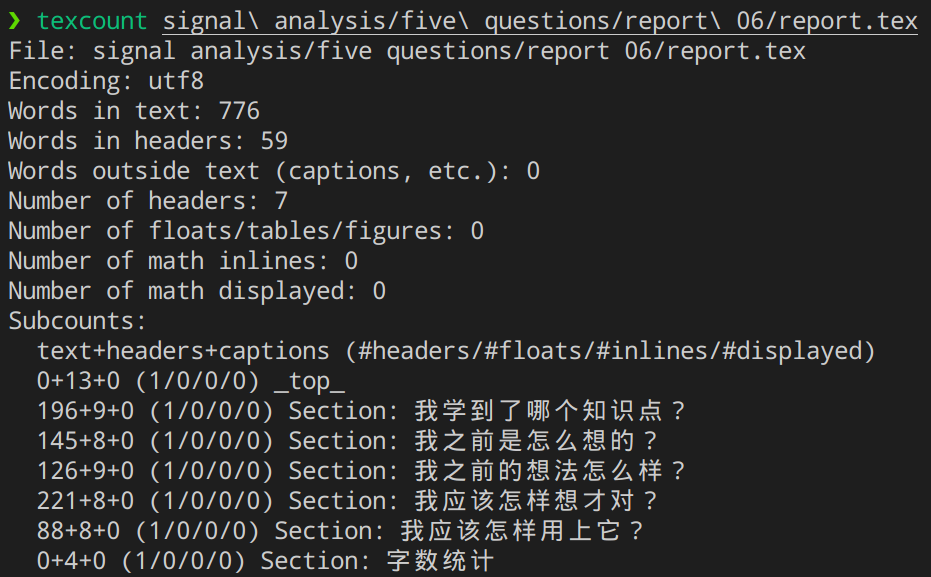
\includegraphics[width=0.8\textwidth]{pics/texcount.png}
    \end{center}

\end{document}